% #############################################################################
% This is Chapter 4
% !TEX root = ../main.tex
% #############################################################################
% Change the Name of the Chapter i the following line
\fancychapter{System Architecture}
\cleardoublepage
% The following line allows to ref this chapter
\label{chap:arch}

The objective of the system was to develop a device in a box format to enable users to establish safe channels of communication. This is achieved with a safe and secure device which is personal to each individual. In order to secure the communications between users, the device saves the user's sensitive data, such as keys, and performs all security critical operations.
The system is designed so that each user has it's own physical box.

% -----------------------------------------------------
% -----------------------------------------------------
\section{Components} \label{chap:arch:components}

%% Insert image "figure"
\begin{figure}[h]
    \centering
    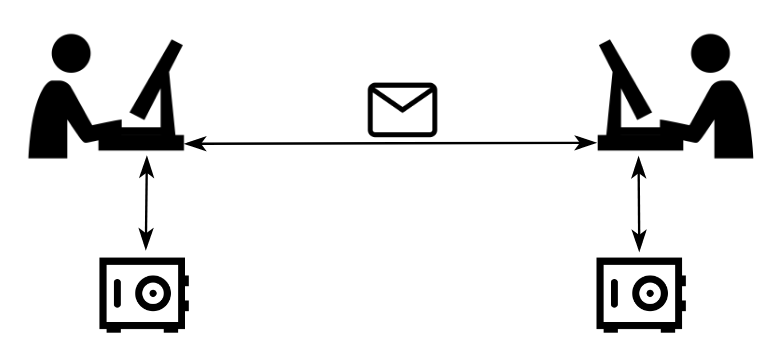
\includegraphics[width=0.5\textwidth]{./Images/main-figure2.png}
    \caption{Client and device}
    \label{fig:main-components}
\end{figure}

The solution is composed of two main components, as shown in figure \ref{fig:main-components}:

\begin{itemize}
    \item The physical box which responsible for securing communications;
    \item The client application on the user's computer which provides an interface for the user to execute operations on the box.
\end{itemize}

By separating these components, the security of the system is isolated and solely of total responsibility of the box. It is not dependent on the user's personal computer.

Both components are connected through a common interface, such as USB, in order to be more easily accessible to the end users.

Figure \ref{fig:securebox} depicts the client application, interacting with the secure device through the \ac{API}, the implementation of operations inside the device and secure storage where all the keys are stored.

% TODO - ADD AT LEAST 3 USERS COMMUNICATING
%% Insert image here
\begin{figure}[h]
    \centering
    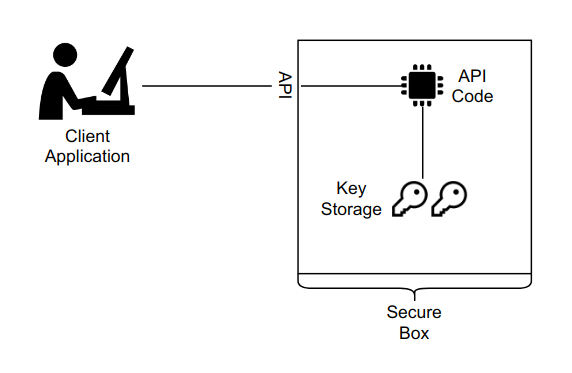
\includegraphics[width=0.5\textwidth]{./Images/securebox.png}
    \caption{Client application and secure device}
    \label{fig:securebox}
\end{figure}

Figure \ref{fig:securebox} depicts the client application, interacting with the secure device through the \ac{API}, the implementation of operations inside the device and secure storage where all the keys are stored.

% -----------------------------------------------------
% -----------------------------------------------------
\section{Operations} \label{chap:arch:ops}

The system operations will ensure the system requirements and services are fulfilled.
For the user to be able to execute them, he first must authenticate himself to the device. This is done with a \ac{PIN} or password, which identifies the user. Once authenticated, the operations will be available to the user to be executed in the box.

The operations are split in three types:
\begin{itemize}
    \item The administration operations manage the authentication and communication configuration;
    \item The data exchange operations secure the user's communication;
    \item The key exchange operations manage the keys stored inside the device, which will be used to secure communications.
\end{itemize}

% -----------------------------------------------------
\subsection{Administration Operations} \label{chap:arch:ops:administration}

The administration operations will allow the user to manage the authentication related parameters.
The only operations of this type is to change the authentication \ac{PIN}. The device will be initialized from fabric with a default \ac{PIN} which must be supplied to the user. Before performing any operation the user should change his PIN to begin secure communications.

% -----------------------------------------------------
\subsection{Data Exchange Operations}  \label{chap:arch:ops:data}

The main operations will be responsible to secure the communications between users. These operations will fulfill the confidentiality, authentication and non-repudiation services.

\begin{itemize}
    \item Secure data exchange with confidentiality and authentication. The objective of this operation is to send and receive data to and from the device. Plaintext data will be returned to the user encrypted and authenticated with their key stored inside the device. In the case of encrypted and authenticated messages, an error will be returned if the decryption was unsuccessful, otherwise, the user will receive the plaintext data;
    \item Digital Signature operation will provide non-repudiation to a piece of data. The user will send the information to the box, and the subsequent signature will be returned, which can be used to verify the data's authorship. To verify a signature, the user sends it to the device, and receives either success or failure to verify.
\end{itemize}

% -----------------------------------------------------
\subsection{Key Exchange Operations}  \label{chap:arch:ops:key}

These operations will handle key exchange when new keys need to be generated and exchanged between users, to enable further communications, and to import other user's public keys. This will serve the secure storage and key management services.

The first operations will enable the user to ask for a new key, generated inside the box, in order to securely send it to another user. The user receiving the new key, generated by another user, will receive and store the key inside the box.
The final operation will provide a way to import other user's public keys, as well as export their personal public key, to be shared with another user.

% -----------------------------------------------------
% -----------------------------------------------------
